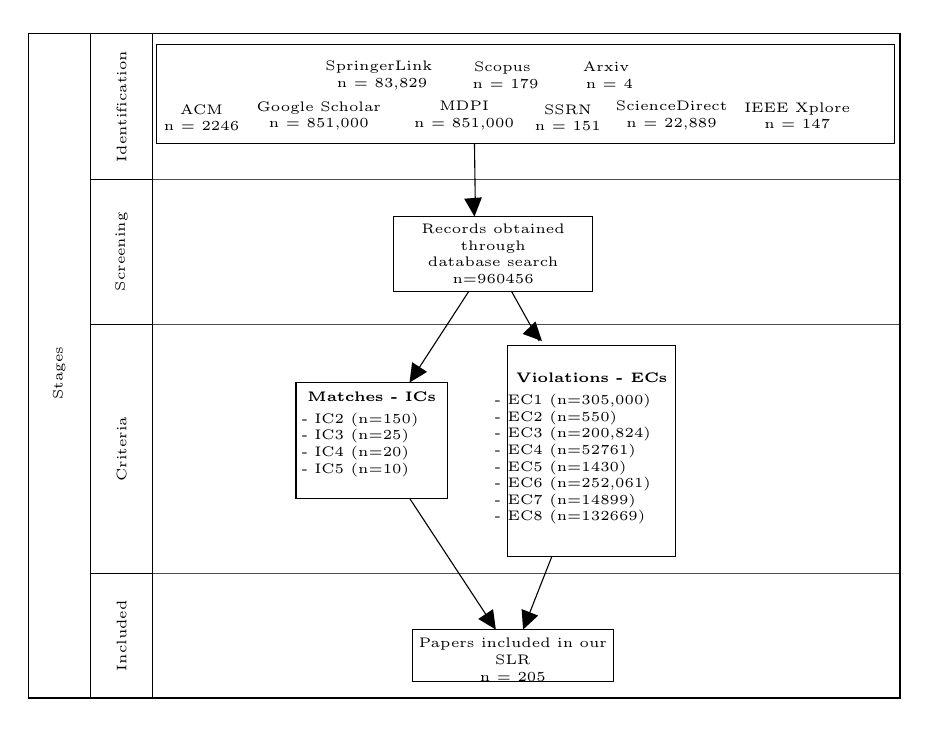
\begin{tikzpicture}[x=0.75pt,y=0.75pt, yscale=-1,xscale=1]
%uncomment if require: \path (0,342); %set diagram left start at 0, and has height of 342

%Shape: Rectangle [id:dp0019014955149456725] 
\draw   (10,10) -- (430,10) -- (430,330) -- (10,330) -- cycle ;

%Shape: Rectangle [id:dp001991157125860177] 
\draw   (10,10) -- (40,10) -- (40,330) -- (10,330) -- cycle ;
%Shape: Rectangle [id:dp904102156184196] 
\draw   (40,10) -- (70,10) -- (70,330) -- (40,330) -- cycle ;
%Shape: Rectangle [id:dp9164832028680756] 
\draw   (40,10) -- (70,10) -- (70,80) -- (40,80) -- cycle ;
%Shape: Rectangle [id:dp844062069727546] 
\draw   (40,80) -- (70,80) -- (70,150) -- (40,150) -- cycle ;
%Shape: Rectangle [id:dp07016298949029287] 
\draw   (40,150) -- (70,150) -- (70,270) -- (40,270) -- cycle ;
%Shape: Rectangle [id:dp5799107359989104] 
\draw   (40,270) -- (70,270) -- (70,330) -- (40,330) -- cycle ;
%Shape: Rectangle [id:dp4056799987768438] 
\draw  [color={rgb, 255:red, 0; green, 0; blue, 0 }  ,draw opacity=0.45 ] (70,10) -- (430,10) -- (430,80) -- (70,80) -- cycle ;
%Shape: Rectangle [id:dp6386898601196207] 
\draw  [color={rgb, 255:red, 0; green, 0; blue, 0 }  ,draw opacity=0.45 ] (70,80) -- (430,80) -- (430,150) -- (70,150) -- cycle ;
%Shape: Rectangle [id:dp2906994943624406] 
\draw  [color={rgb, 255:red, 0; green, 0; blue, 0 }  ,draw opacity=0.45 ] (70,150) -- (430,150) -- (430,270) -- (70,270) -- cycle ;
%Shape: Rectangle [id:dp23551377863706668] 
\draw  [color={rgb, 255:red, 0; green, 0; blue, 0 }  ,draw opacity=0.45 ] (70,270) -- (430,270) -- (430,330) -- (70,330) -- cycle ;

% Text Node
\draw    (72,15) -- (427.5,15) -- (427.5,63) -- (72,63) -- cycle  ;
\draw (93.5,50.5) node  [font=\tiny] [align=left] {\begin{minipage}[lt]{50.33pt}\setlength\topsep{0pt}
\begin{center}
ACM \\ n = 2246
 % Google Scholar Scopus SSRN ScienceDirect MDPI IEEE Xplore SpringerLink 
\end{center}

 \end{minipage}};
% Text Node
% \draw    (121,37) -- (185,37) -- (185,62) -- (121,62) -- cycle  ;
\draw (150,49.5) node  [font=\tiny] [align=left] {\begin{minipage}[lt]{50.24pt}\setlength\topsep{0pt}
\begin{center}
Google Scholar\\n = 851,000
\end{center}

 \end{minipage}};

\draw (220,49.5) node  [font=\tiny] [align=left] {\begin{minipage}[lt]{50.24pt}\setlength\topsep{0pt}
\begin{center}
MDPI\\n = 851,000
\end{center}

 \end{minipage}};
 
% Text Node
\draw (270,50.5) node  [font=\tiny] [align=left] {\begin{minipage}[lt]{50.59pt}\setlength\topsep{0pt}
\begin{center}
SSRN\\n = 151 
\end{center}

\end{minipage}};
% Text Node
\draw (320,49.5) node  [font=\tiny] [align=left] {\begin{minipage}[lt]{50.12pt}\setlength\topsep{0pt}
\begin{center}
ScienceDirect \\n = 22,889
\end{center}

\end{minipage}};
% Text Node
\draw (380.5,49.5) node  [font=\tiny] [align=left] {\begin{minipage}[lt]{50.26pt}\setlength\topsep{0pt}
\begin{center}
IEEE Xplore \ \\n = 147
\end{center}

\end{minipage}};
% Text Node
\draw (180.5,30) node  [font=\tiny] [align=left] {\begin{minipage}[lt]{50.88pt}\setlength\topsep{0pt}
\begin{center}
SpringerLink \ \ \\n = 83,829
\end{center}

\end{minipage}};

% Text Node
\draw (240,30) node  [font=\tiny] [align=left] {\begin{minipage}[lt]{50.88pt}\setlength\topsep{0pt}
\begin{center}
Scopus \ \ \\n = 179
\end{center}

\end{minipage}};

% Text Node
\draw (290,30) node  [font=\tiny] [align=left] {\begin{minipage}[lt]{50.88pt}\setlength\topsep{0pt}
\begin{center}
Arxiv \ \ \\n = 4
\end{center}

\end{minipage}};




% Text Node
\draw    (186,98) -- (282,98) -- (282,134) -- (186,134) -- cycle  ;
\draw (234,116) node  [font=\tiny] [align=left] {\begin{minipage}[lt]{62.52pt}\setlength\topsep{0pt}
\begin{center}
Records obtained through \\database search \\n=960456
\end{center}

\end{minipage}};

%\draw    (186,98) -- (282,98) -- (282,134) -- (186,134) -- cycle  ;
%\draw (400,116) node  [font=\tiny] [align=left] {\begin{minipage}[lt]{62.52pt}\setlength\topsep{0pt}
%\begin{center}
%Records obtained through \\database search \\n=960456
%\end{center}

%\end{minipage}};
% Text Node
\draw (25,173.5) node  [font=\tiny,rotate=-270] [align=left] {\begin{minipage}[lt]{50.39pt}\setlength\topsep{0pt}
\begin{center}
Stages
\end{center}

\end{minipage}};
% Text Node
\draw (55,45) node  [font=\tiny,rotate=-270] [align=left] {\begin{minipage}[lt]{50.31pt}\setlength\topsep{0pt}
\begin{center}
Identification
\end{center}

\end{minipage}};
% Text Node
\draw (55,115) node  [font=\tiny,rotate=-270] [align=left] {\begin{minipage}[lt]{50.24pt}\setlength\topsep{0pt}
\begin{center}
Screening
\end{center}

\end{minipage}};
% Text Node
\draw (55,210) node  [font=\tiny,rotate=-270] [align=left] {\begin{minipage}[lt]{50.12pt}\setlength\topsep{0pt}
\begin{center}
Criteria
\end{center}

\end{minipage}};
% Text Node
\draw (55,300) node  [font=\tiny,rotate=-270] [align=left] {\begin{minipage}[lt]{50.1pt}\setlength\topsep{0pt}
\begin{center}
Included
\end{center}

\end{minipage}};
% Text Node
\draw    (139,178) -- (212,178) -- (212,234) -- (139,234) -- cycle  ;
\draw (175.5,206) node  [font=\tiny] [align=left] {\begin{minipage}[lt]{50.71pt}\setlength\topsep{0pt}
\begin{center}
\textbf{Matches - ICs} 
\end{center}
- IC2 (n=150)\\
- IC3 (n=25)\\
- IC4 (n=20)\\
- IC5 (n=10) \\
% - IC3 (n=\hl{15})\\
% - IC4 (n=\hl{14})\\
% - IC5 (n=\hl{5})\\
% - IC6 (n=\hl{19}) \\
\end{minipage}};
% Text Node
\draw    (241,160) -- (322,160) -- (322,262) -- (241,262) -- cycle  ;
\draw (281.5,213) node  [font=\tiny] [align=left] {\begin{minipage}[lt]{70.21pt}\setlength\topsep{0pt}
\begin{center}
\textbf{Violations - ECs}
\end{center}
- EC1 (n=305,000)\\
- EC2 (n=550)\\
- EC3 (n=200,824)\\ % 2062 + 1 secondary study (Caulo et al.)
- EC4 (n=52761)\\
- EC5 (n=1430)\\
- EC6 (n=252,061)\\
- EC7 (n=14899)\\
- EC8 (n=132669)\\
\end{minipage}};
% Text Node
\draw    (195,297) -- (292,297) -- (292,322) -- (195,322) -- cycle  ;
\draw (243.5,311.5) node  [font=\tiny] [align=left] {\begin{minipage}[lt]{80.33pt}\setlength\topsep{0pt}
\begin{center}
Papers included in our SLR\\n = 205
\end{center}

\end{minipage}};
% Connection
%\draw    (112,59.12) -- (192.67,96.73) ;
%\draw [shift={(195.39,98)}, rotate = 204.99] [fill={rgb, 255:red, 0; green, 0; blue, 0 }  ][line width=0.08]  [draw opacity=0] (8.93,-4.29) -- (0,0) -- (8.93,4.29) -- cycle    ;
% Connection
%\draw    (168.23,62) -- (209.76,96.1) ;
%\draw [shift={(212.08,98)}, rotate = 219.39] [fill={rgb, 255:red, 0; green, 0; blue, 0 }  ][line width=0.08]  [draw opacity=0] (8.93,-4.29) -- (0,0) -- (8.93,4.29) -- cycle    ;
% Connection
\draw    (225,63) -- (225.44,95.23) ;
\draw [shift={(225,98)}, rotate = 265.6] [fill={rgb, 255:red, 0; green, 0; blue, 0 }  ][line width=0.1]  [draw opacity=0] (8.93,-4.29) -- (0,0) -- (8.93,4.29) -- cycle    ;
% Connection
%\draw    (258.36,62) -- (243.35,95.27) ;
%\draw [shift={(242.12,98)}, rotate = 294.28] [fill={rgb, 255:red, 0; green, 0; blue, 0 }  ][line width=0.08]  [draw opacity=0] (8.93,-4.29) -- (0,0) -- (8.93,4.29) -- cycle    ;
% Connection
%\draw    (310.74,62) -- (262.03,96.27) ;
%\draw [shift={(259.58,98)}, rotate = 324.87] [fill={rgb, 255:red, 0; green, 0; blue, 0 }  ][line width=0.08]  [draw opacity=0] (8.93,-4.29) -- (0,0) -- (8.93,4.29) -- cycle    ;
% Connection
%\draw    (358,61.57) -- (277.75,96.79) ;
%\draw [shift={(275.01,98)}, rotate = 336.3] [fill={rgb, 255:red, 0; green, 0; blue, 0 }  ][line width=0.08]  [draw opacity=0] (8.93,-4.29) -- (0,0) -- (8.93,4.29) -- cycle    ;
% Connection
\draw    (222.3,134) -- (195.33,175.48) ;
\draw [shift={(193.7,178)}, rotate = 303.02] [fill={rgb, 255:red, 0; green, 0; blue, 0 }  ][line width=0.08]  [draw opacity=0] (8.93,-4.29) -- (0,0) -- (8.93,4.29) -- cycle    ;
% Connection
\draw    (242.81,134) -- (256.19,158) ;
\draw [shift={(257.51,158)}, rotate = 225.91] [fill={rgb, 255:red, 0; green, 0; blue, 0 }  ][line width=0.08]  [draw opacity=0] (8.93,-4.29) -- (0,0) -- (8.93,4.29) -- cycle    ;
% Connection
\draw    (193.9,234) -- (233.64,294.49) ;
\draw [shift={(235.29,297)}, rotate = 236.69] [fill={rgb, 255:red, 0; green, 0; blue, 0 }  ][line width=0.08]  [draw opacity=0] (8.93,-4.29) -- (0,0) -- (8.93,4.29) -- cycle    ;
% Connection
\draw    (262.2,262) -- (249.52,294.21) ;
\draw [shift={(248.42,297)}, rotate = 291.49] [fill={rgb, 255:red, 0; green, 0; blue, 0 }  ][line width=0.08]  [draw opacity=0] (8.93,-4.29) -- (0,0) -- (8.93,4.29) -- cycle;

\end{tikzpicture}
